\section{Application 1: Whitening Variational Gaussian Processes}
\label{sec:variational_results}

\gp{Lead in here.}

Assume we have $M$ inducing points $\bZ = [\bz_1, \ldots, \bz_m]$.
Let $q(\bu) = \normaldist{\bu; \bm}{\bS}$ be the approximate function distribution at the inducing points $\bZ$.
For an arbitrary point $\bxtest$, the predictive distribution for the approximate Gaussian process is given by
%
\begin{equation}
  q \left( f(\bxtest) \right) = \Evover{q(\bu)}{ \: p\left( f(\bxtest) \mid \bu \right) \: }
  = \normaldist{ \bxtest; \ameantest{ \bxtest }} { \avartest{ \bxtest }}
  \label{eqn:approx_pred}
\end{equation}
%
where $\ameantest{\cdot}$ and $\avartest{\cdot}$ are the (approximate) predictive mean and covariance functions, given by:
%
\begin{align}
  \ameantest{\bxtest} &= \bk_{\bZ\bxtest}^\top \bK_{\bZ\bZ}^{-1} \bm
  \label{eqn:approx_pred_mean} \\
  \avartest{\bxtest} &= k(\bxtest, \bxtest) -
    \bk_{\bZ\bxtest}^\top \bK_{\bZ\bZ}^{-1} \left( \bK_{\bZ\bZ} - \bS \right) \bK_{\bZ\bZ}^{-1} \bk_{\bZ\bxtest}
  \label{eqn:approx_pred_covar}
\end{align}
%
and the parameters $\bm$ and $\bS$ (as well as the inducing locations $\bZ$ and associated kernel/likelihood hyperparameters) optimize the variational evidence-lower bound (ELBO):
%
\begin{align}
	-\loglik_\text{ELBO} = -\sum_{i=1}^N \Evover{q(f(\bx^{(i)}))}{  \: \log p( y^{(i)} \mid f(\bx^{(i)}) ) \: } + \kl{ q(\bu) }{ p(\bu) },
	\label{eqn:elbo}
	\nonumber
\end{align}
%
%The KL divergence is minimized when $\bm = \bzero$ and $\bS = \bK_{\bZ\bZ}$.
Rather than directly learning $\bm$ and $\bS$, it is more common to learn the \emph{whitened parameters} \cite{kuss2005assessing,matthews2017scalable}:
\[ \bm' = \bK^{-\frac 1 2} \bm, \quad \bS' = \bK^{-\frac 1 2} \bS \bK^{-\frac 1 2} \]
Under this coordinate system, the KL divergence term is given by
%
\begin{equation}
	\kl{ q(\bu') }{ p(\bu') } = \frac{1}{2} \Bigl( \bm^{\prime \top} \bm' + \tr{ \bS' } - \log \vert \bS' \vert - M \Bigr),
	\label{eqn:kldiv_whitened}
\end{equation}
%
which importantly does not depend on $k(\cdot,\cdot)$ or $\bZ$ and therefore is relatively simple to optimize.
The whitened predictive mean and variance become
%
\begin{align}
  \ameantest{\bxtest} &= \bk_{\bZ\bxtest}^\top \bK^{-\frac 1 2} \bm'
  \label{eqn:approx_pred_mean} \\
  \avartest{\bxtest} &= k(\bxtest, \bxtest) -
    \bk_{\bZ\bxtest}^\top \bK^{-\frac 1 2} \left( \bI - \bS' \right) \bK^{-\frac 1 2} \bk_{\bZ\bxtest}
  \label{eqn:approx_pred_covar}
\end{align}

During optimization, we must compute the predictive distribution of every data point $\bx_i, y_i$.
This requires computing $\bK^{- \frac 1 2} \bk_{\bX \bx_i}$ and its derivative for every $\bx_i$ at every optimization iteration.\footnote{
  Since SVGP is compatible with minibatch optimization, we often only compute $\bK^{- \frac 1 2} \bk_{\bZ \bx_i}$ for a fraction of the training data.
}
This can computed using the Cholesky decomposition (up to an orthogonal rotation) or CIQ.

\gp{Stopped here.}

\begin{figure}[t!]
  \centering
  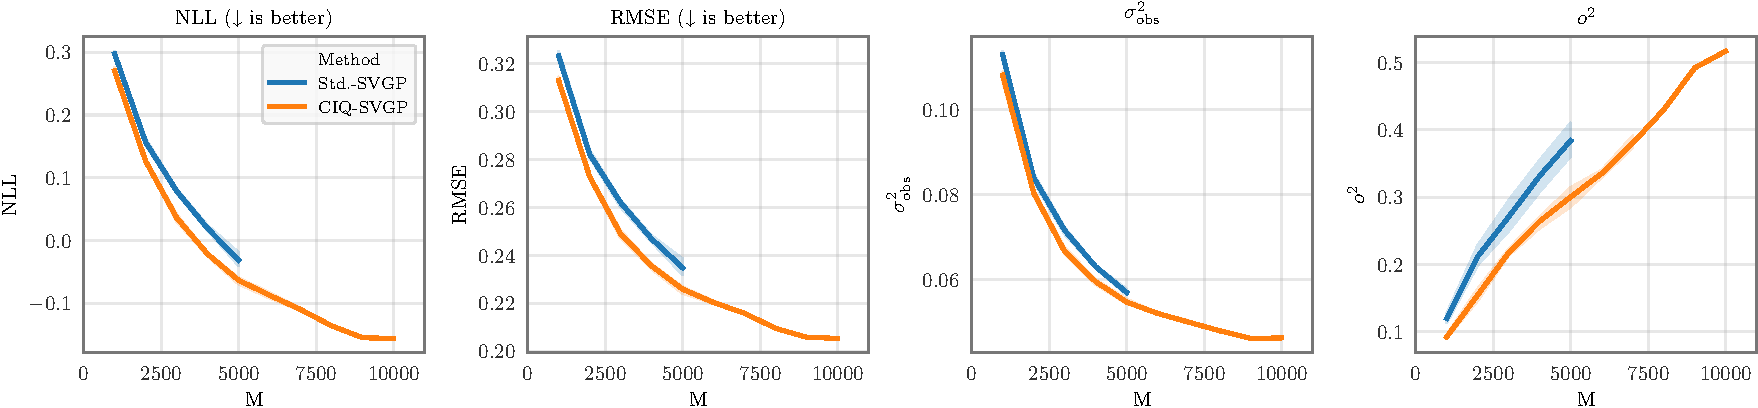
\includegraphics[width=\linewidth]{figures/3droad.pdf}
  \caption{
    SVGP models trained on the 3D-Road dataset ($D=2$, $N\geq300,\!000$), varying $M$ (the number of inducing points).
    \gp{FINISH}
  }
  \label{fig:3droad}
\end{figure}

\begin{figure}[t!]
  \centering
  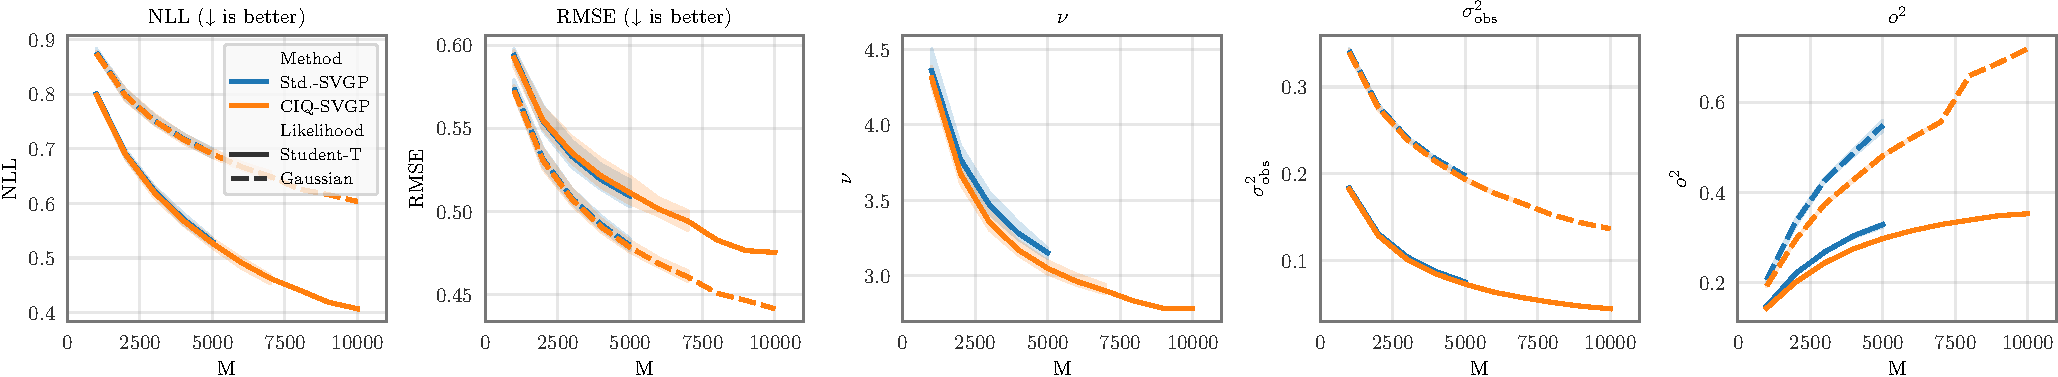
\includegraphics[width=\linewidth]{figures/precip.pdf}
  \caption{
    SVGP models trained on the Precipitation dataset ($D=3$, $N\geq300,\!000$), varying $M$ (the number of inducing points).
    \gp{FINISH}
  }
  \label{fig:precip}
\end{figure}

\begin{figure}[t!]
  \centering
  \caption{
    SVGP models trained on the Robotics dataset ($D=?$, $N\geq?$), varying $M$ (the number of inducing points).
    \gp{FINISH}
  }
  \label{fig:robotics}
\end{figure}
